%! Author = adnansiddiquei
%! Date = 13/12/2023

\subsection{Q2 - Dataset B}\label{subsec:dataset-b}
    \begin{figure}
    \centering
    \begin{subfigure}{0.9\textwidth}
      \centering
      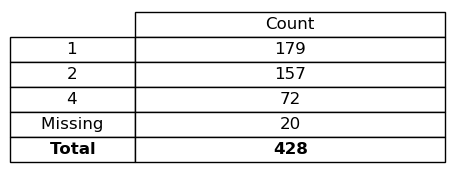
\includegraphics[width=.55\linewidth]{./figures/q2a}
      \caption{Raw \inlinecode{B_NoiseAdded.csv} dataset, before pre-processing. There are 428 observations with 20 missing
        labels and 20 duplicated observations (40 observations involved in the duplication).}
      \label{fig:q2a}
    \end{subfigure}%
    \hfill
    \begin{subfigure}{0.9\textwidth}
      \centering
      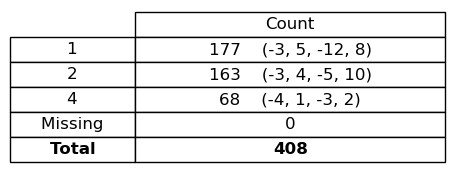
\includegraphics[width=0.55\linewidth]{./figures/q2b_q2d}
      \caption{\inlinecode{B_NoiseAdded.csv} after pre-processing, no missing labels or duplicated observations.
        The 4 numbers in the brackets indicate how the count in each classification changed due to, in order: 1 and 2
        are counts exiting and entering (respectively) the class after correcting for mislabelling; 3 -
        count exiting after dropping duplicates; 4 - count entering after imputation of missing labels.}
      \label{fig:q2bd}
    \end{subfigure}
    \caption{Summary of classifications for the \inlinecode{B_NoiseAdded.csv} dataset before and after pre-processing.}
    \label{fig:q2abd}
    \end{figure}

    Fig.\eqref{fig:q2a} summarises the classifications for \inlinecode{B_NoiseAdded.csv}.
    The dataset contained 20 duplicates (40 involved in the duplication, full list in Appendix \ref{appendix:q2}) and
    20 missing labels.
    10 of these 20 duplicates were also mislabelled, as they contained mismatched labels across their duplicates.
    A multinomial \inlinecode{LogisticRegression} model was fit on the labelled data to predict the missing and mislabelled
    labels, Fig.\eqref{fig:q2bd} shows the new summary of classifications.

    Several methods exist for handling missing labels.
    One method, model based imputation (used here), involves training a model on labelled data to predict missing labels.
    Alternatively, data with missing labels can be ignored, especially if the sample size is large.
    Whilst model based imputation utilises all data, it risks bias if the model poorly fits the data.
    Ignoring missing data avoids bias, if the samples size is large.

    Missing at random (MAR) means a label's absence is unrelated to its value, whereas missing not at random (MNAR)
    indicates a correlation between a label's absence and its value.
    In Fig.\eqref{fig:q2bd}, the missing labels' percentages in each class (4.5\%, 6.1\%, and 2.9\% for classes 1, 2,
    and 4) suggest no significant evidence of MNAR.
